\section{Histoire du DICOM}

	\frame
	{
		\frametitle{Pr\'ehistoire}
		
		\begin{itemize}
			\item Arriv\'ee du num\'erique en m\'edecine.
			\item Stockage, transmission, affichage des images : constructeur d\'ependant.
			\item Solutions propri\'etaires (par opposition \`a solutions ouvertes) :
			\begin{itemize}
				\item argument commercial : "Mon protocole est meilleur que les autres", "Nos produits ont une excellente interaction entre eux", "Nous g\'erons tout de A \`a Z" ;
				\item interaction impossible entre marques diff\'erentes.
			\end{itemize} 
			\item Cons\'equences :
			\begin{itemize}
				\item pi\`ege commercial : obligation d'acqu\'erir les stations d'acquisition et de traitement ad\'equates, et changer de marque peut rendre les anciens examens illisibles ;
				\item pi\`ege m\'edical : difficile de communiquer entre coll\`egues.
			\end{itemize}
		\end{itemize}
	}
					
	\frame
	{
		\frametitle{D\'ebuts du DICOM}
		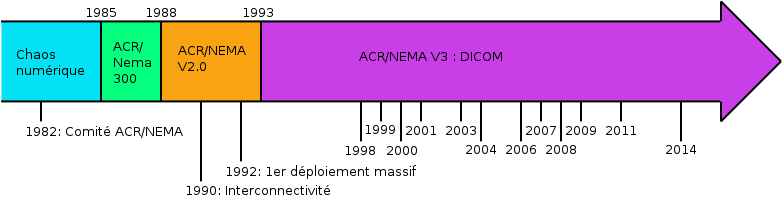
\includegraphics[width=\linewidth]{./figures/chrono-dicom.png}

		\begin{itemize}
			\item 1\up{\`ere} version ACR/NEMA 300 en 1985 : peu accept\'e car vague et contenant des incoh\'erences.
			\item 2\up{\`eme} version en 1988 : transmission des images par le connecteur mat\'eriel EIA-485, adopt\'e par quelques constructeurs.
			\item 3\up{\`eme} version en 1993 : ind\'ependance du connecteur, donc support TCP.
		\end{itemize}
	}
	
	\frame
	{
		\frametitle{Support / Sponsoring}
		\begin{itemize}
			\item ACR : American College of Radiology
			\item NEMA : National Electrical Manufacturers Association
			\item JIRA : Japan Investor Relations Association
			\item CEN : Comit\'e Europ\'een de Normalisation
			\item IEEE, HL7, ANSI,\ldots
		\end{itemize}
	}

	\frame
	{
		\frametitle{DICOM aujourd'hui}
		\begin{itemize}
			\item Standard accept\'e mondialement.
			\item Actuellement en version $2014b$ : on parle des versions par leur ann\'ee (officiellement, toujours en version 3, ou PS3)
			\item Diversit\'e des \'equipements support\'es : RX, CT, IRM, US, PET, SPECT, Angio, ECG,\ldots
			\item Adopt\'e par de nombreux constructeurs : GE, Siemens, Philips, Toshiba,\ldots
		\end{itemize}
	}
